\chapter{Appendix}
\addtocontents{toc}{\protect\setcounter{tocdepth}{-1}}
%
To quantify the mismatches of proton MC simulations and observed data, a random
forest is trained on the feature set, implemented in the \texttt{FeatureStream}, to distinguish the both. Since the
observed data vastly consists of hadron events, for a perfect simulation it
should hardly be possible to distinguish the data sets, while for existing
mismatches, the AUC of the model quantifies those. The ROC curve is shown in \autoref{fig:mcd_roc}. The resulting AUC of
0.7509\,\pm\,0.0025 is very high and therefore represents a good
discrimination. An AUC this large thus indicates strong data MC mismatches.
%
\begin{figure}
  \centering
  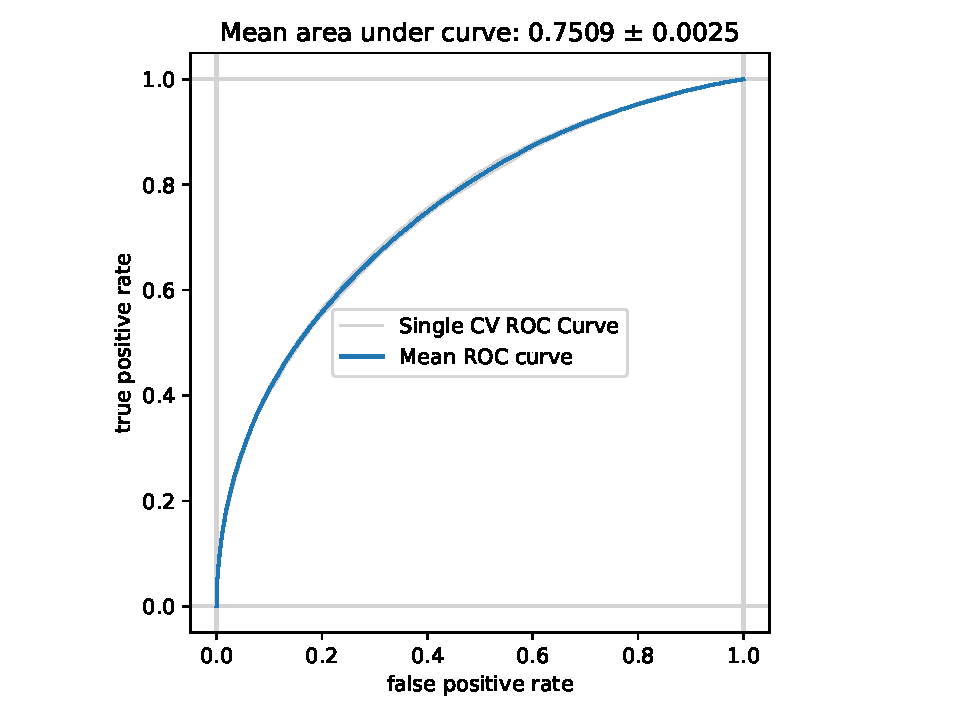
\includegraphics[width=\textwidth]{Plots/data_mc/data_mc_separation.pdf}
  \caption{ROC curve for a random forest model discriminating between proton MC simulations and observed data based in the features implemented in the \texttt{FeatureStream}. The resulting AUC of 0.7509\,\pm\,0.0025 is very high and therefore represents a good discrimination. The proton MC simulations are supposed to model the vast majority of observed data, since the hadron flux is dominating. An AUC this large thus indicates strong data MC mismatches.}
  \label{fig:mcd_roc}
\end{figure}
%

%
\begin{figure}
  \begin{subfigure}{0.5\textwidth}
    \centering
    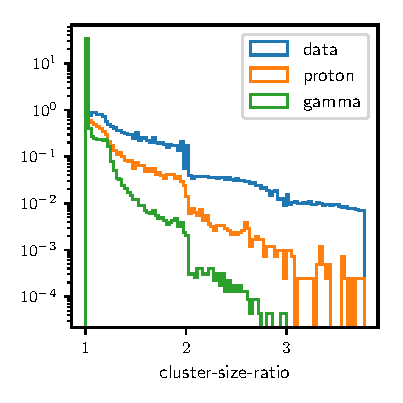
\includegraphics[width=\textwidth, page=1]{Plots/data_mc/features_DBSCAN.pdf}
  \end{subfigure}
  \begin{subfigure}{0.5\textwidth}
    \centering
    \includegraphics[width=\textwidth, page=2]{Plots/data_mc/features_DBSCAN.pdf}
  \end{subfigure}
  \begin{subfigure}{0.5\textwidth}
    \centering
    \includegraphics[width=\textwidth, page=3]{Plots/data_mc/features_DBSCAN.pdf}
  \end{subfigure}
  \begin{subfigure}{0.5\textwidth}
    \centering
    \includegraphics[width=\textwidth, page=4]{Plots/data_mc/features_DBSCAN.pdf}
  \end{subfigure}
  \caption{Features of the reconstructed air-showers using the DBSCAN cleaning. The blue histograms show the observed data, whereas orange and green show proton and gamma MC simulations respectively. The histograms are normalized to the respective observation time or simulated observation time.}
\end{figure}
%
%
\begin{figure}
  \begin{subfigure}{0.5\textwidth}
    \centering
    \includegraphics[width=\textwidth, page=5]{Plots/data_mc/features_DBSCAN.pdf}
  \end{subfigure}
  \begin{subfigure}{0.5\textwidth}
    \centering
    \includegraphics[width=\textwidth, page=6]{Plots/data_mc/features_DBSCAN.pdf}
  \end{subfigure}
  \begin{subfigure}{0.5\textwidth}
    \centering
    \includegraphics[width=\textwidth, page=7]{Plots/data_mc/features_DBSCAN.pdf}
  \end{subfigure}
  \begin{subfigure}{0.5\textwidth}
    \centering
    \includegraphics[width=\textwidth, page=8]{Plots/data_mc/features_DBSCAN.pdf}
  \end{subfigure}
  \caption{Features of the reconstructed air-showers using the DBSCAN cleaning. The blue histograms show the observed data, whereas orange and green show proton and gamma MC simulations respectively. The histograms are normalized to the respective observation time or simulated observation time.}
\end{figure}
%
%
\begin{figure}
  \begin{subfigure}{0.5\textwidth}
    \centering
    \includegraphics[width=\textwidth, page=9]{Plots/data_mc/features_DBSCAN.pdf}
  \end{subfigure}
  \begin{subfigure}{0.5\textwidth}
    \centering
    \includegraphics[width=\textwidth, page=13]{Plots/data_mc/features_DBSCAN.pdf}
  \end{subfigure}
  \begin{subfigure}{0.5\textwidth}
    \centering
    \includegraphics[width=\textwidth, page=14]{Plots/data_mc/features_DBSCAN.pdf}
  \end{subfigure}
  \begin{subfigure}{0.5\textwidth}
    \centering
    \includegraphics[width=\textwidth, page=15]{Plots/data_mc/features_DBSCAN.pdf}
  \end{subfigure}
  \caption{Features of the reconstructed air-showers using the DBSCAN cleaning. The blue histograms show the observed data, whereas orange and green show proton and gamma MC simulations respectively. The histograms are normalized to the respective observation time or simulated observation time.}
\end{figure}
%
%
\begin{figure}
  \begin{subfigure}{0.5\textwidth}
    \centering
    \includegraphics[width=\textwidth, page=16]{Plots/data_mc/features_DBSCAN.pdf}
  \end{subfigure}
  \begin{subfigure}{0.5\textwidth}
    \centering
    \includegraphics[width=\textwidth, page=17]{Plots/data_mc/features_DBSCAN.pdf}
  \end{subfigure}
  \begin{subfigure}{0.5\textwidth}
    \centering
    \includegraphics[width=\textwidth, page=18]{Plots/data_mc/features_DBSCAN.pdf}
  \end{subfigure}
  \begin{subfigure}{0.5\textwidth}
    \centering
    \includegraphics[width=\textwidth, page=19]{Plots/data_mc/features_DBSCAN.pdf}
  \end{subfigure}
  \caption{Features of the reconstructed air-showers using the DBSCAN cleaning. The blue histograms show the observed data, whereas orange and green show proton and gamma MC simulations respectively. The histograms are normalized to the respective observation time or simulated observation time.}
\end{figure}
%
%
\begin{figure}
  \begin{subfigure}{0.5\textwidth}
    \centering
    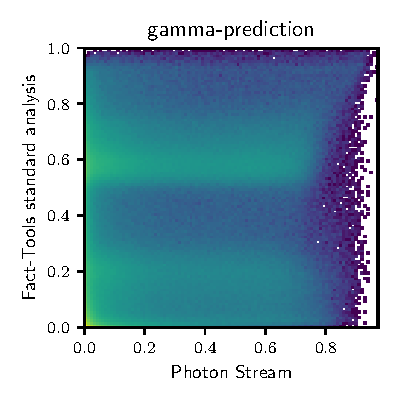
\includegraphics[width=\textwidth, page=1]{Plots/comparison_data_dl3.pdf}
  \end{subfigure}
  \begin{subfigure}{0.5\textwidth}
    \centering
    \includegraphics[width=\textwidth, page=2]{Plots/comparison_data_dl3.pdf}
  \end{subfigure}
  \begin{subfigure}{0.5\textwidth}
    \centering
    \includegraphics[width=\textwidth, page=3]{Plots/comparison_data_dl3.pdf}
  \end{subfigure}
  \begin{subfigure}{0.5\textwidth}
    \centering
    \includegraphics[width=\textwidth, page=4]{Plots/comparison_data_dl3.pdf}
  \end{subfigure}
  \caption{Features of the reconstructed air-showers and output of the separation random forest for PhotonStream data using the DBSCAN cleaning and the FACT-Tools analysis. The scatter plots show the features on observations for the same events. The FACT-Tools results are shown on the y-axis, while the PhotonStream data is on the x-axis.}
\end{figure}
%
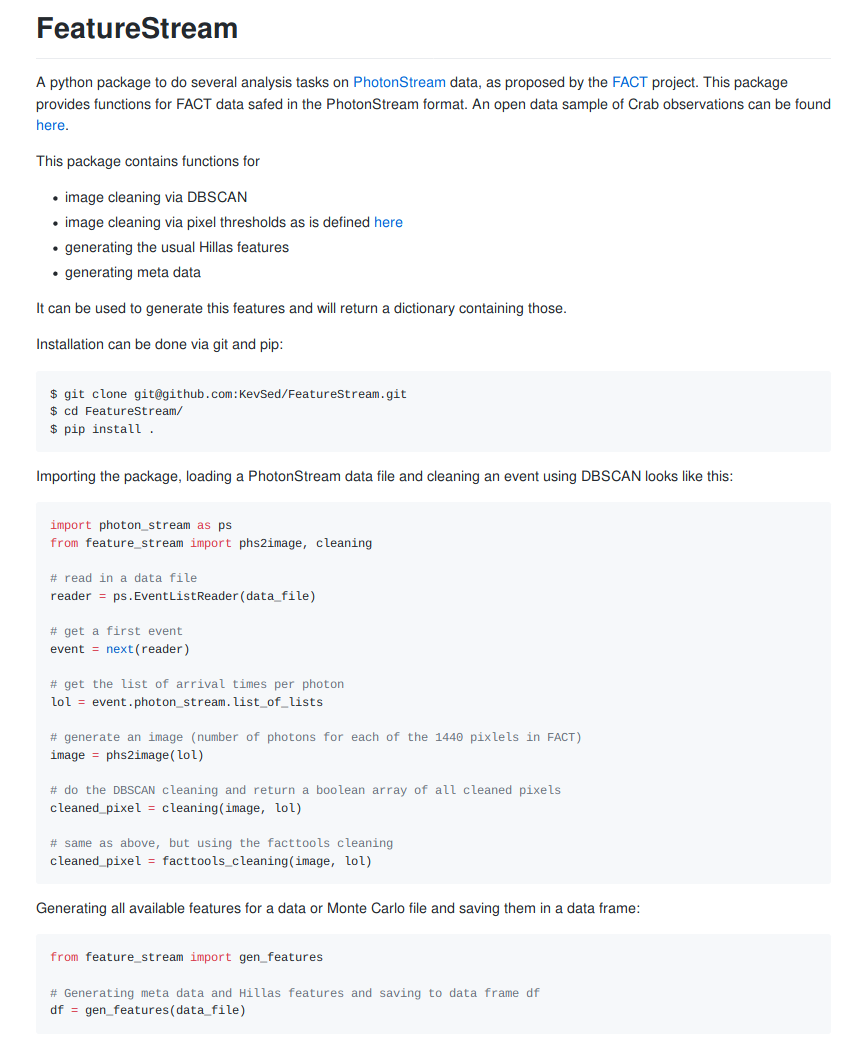
\includegraphics[width=1.2\textwidth]{Plots/feature_stream_readme.png}

%
The energy bias and resolution of the analysis are shown for bins of true gamma
energy in \autoref{fig:bias}.
%
\begin{figure}
  \centering
  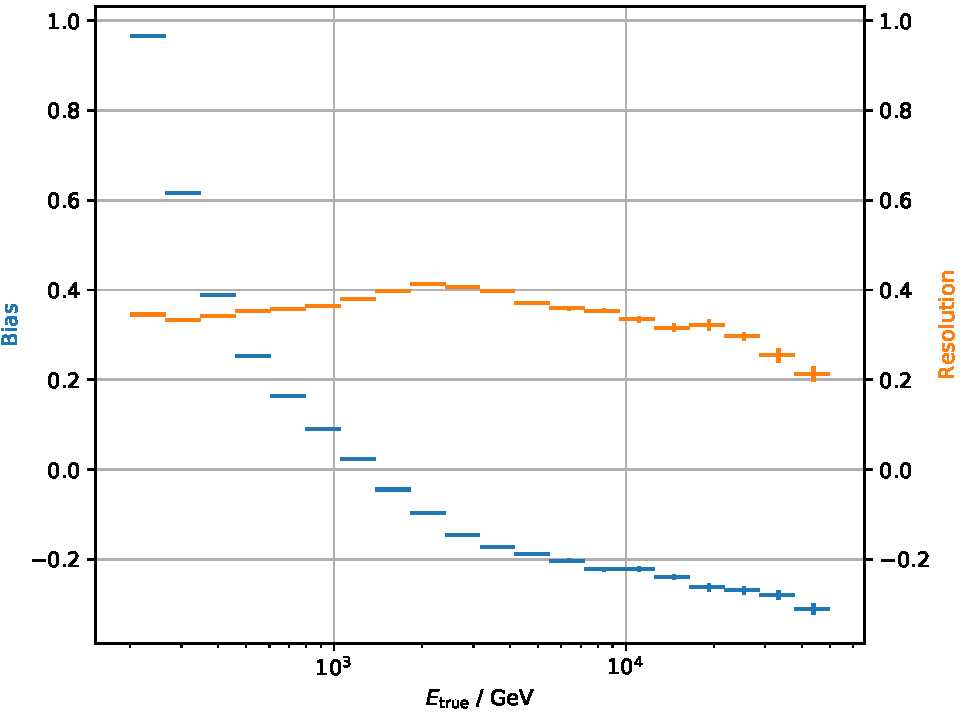
\includegraphics[width=0.9\textwidth]{Plots/results/DBSCAN/bias_resolution.pdf}
  \caption{Bias (blue histogram) and resolution (orange histogram) of the PhotonStream data on DBSCAN cleaning as a function of true Energy of the gamma rays.}
  \label{fig:bias}
\end{figure}
%

\begin{figure}
  \centering
  \includegraphics[width=0.9\textwidth, page=2]{Plots/results/DBSCAN/separation_performance.pdf}
  \caption{Distributions of the gamma confidence for proton and MC simulations of the random forest used for the gamma hadron separation.}
\end{figure}
%
\begin{figure}
  \centering
  \includegraphics[width=0.9\textwidth, page=3]{Plots/results/DBSCAN/separation_performance.pdf}
  \caption{Distributions of the precision, recall and $f_{0.10}$ score of the random forest used for the gamma hadron separation.}
\end{figure}

\addtocontents{toc}{\protect\setcounter{tocdepth}{0}}
